\section{研究目的}
%
今回対象とするカテゴリの投稿例を今回扱ったデータセットから抜粋したものが以下の図\ref{fig:examples}である.

\begin{figure}[ht]
    \centering
    \begin{subfigure}[b]{0.4\textwidth}
        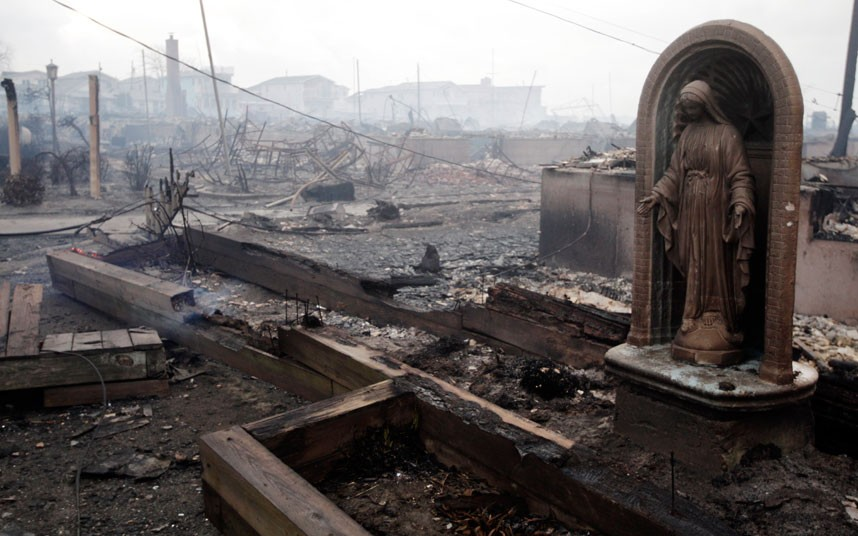
\includegraphics[width=6cm]{images/real_example.jpg}
        \caption{Recovering From Sandy: Breezy Point, Queens; Santiago, Cuba}
        \label{fig:real}
    \end{subfigure}
    \hfill % separation between the subfigures
    \begin{subfigure}[b]{0.4\textwidth}
        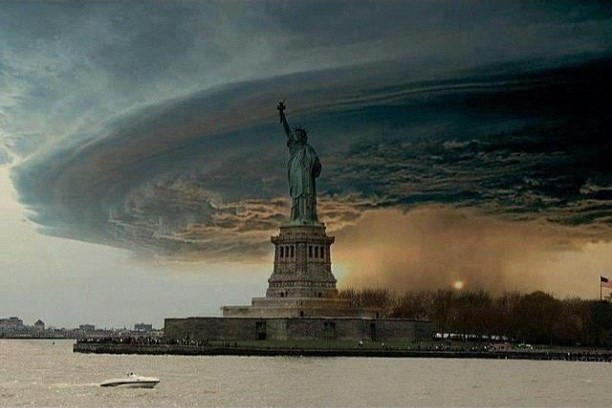
\includegraphics[width=6cm]{images/fake_example.jpg}
        \caption{New York gonna be screwed \#sandy \#hurricane \#newyork \#fucked}
        \label{fig:fake}
    \end{subfigure}
    \hfill % separation between the subfigures
    \begin{subfigure}[b]{0.4\textwidth}
        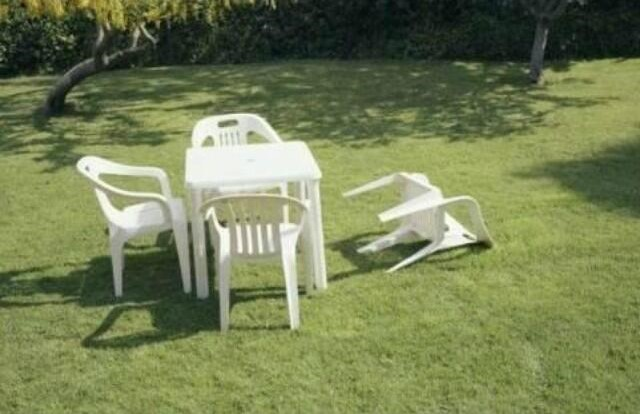
\includegraphics[width=6cm]{images/humor_example.jpg}
        \caption{Britain's last hurricane was devastating...}
        \label{fig:humor}
    \end{subfigure}
    \caption{当研究で扱う3カテゴリの投稿例: (a)正しいニュース,(b)フェイクニュース,(c)ジョークニュース}
    \label{fig:examples}
\end{figure}

いずれも2012年に発生したハリケーン・サンディに関してTwitter上で投稿されたものであった.
図\ref{fig:real}は実際に撮影された被害を免れた聖母マリア像を写したもの,
図\ref{fig:fake}は2004年に撮影された写真に自由の女神を合成させたもの\cite{harmanci_2012},
図\ref{fig:humor}はイギリスにハリケーンが来ないことを茶化すものである.

%
当研究では,上記対象を正確に3カテゴリへ分類するモデルを構築することを目標としている.
具体的には,入力として画像と文章を持ち,それに対してどのカテゴリが該当するかを出力するモデルとなる.

当研究を更に発展させると,SNS上でユーザや運営側を支援するエージェント開発に繋げることができる.
%